\documentclass[a4paper,12pt]{article}
\usepackage{graphicx}
\usepackage[hyphens]{url}
\usepackage{hyperref}
\title{COMP3210 Advanced Computer Networking --- Mesh Networking Chat Program
proposal}
\author{Murray Colpman --- mwrc1g12; Alex Lay --- acl1g12}
\begin{document}
\maketitle

\section{Summary}

We propose to build a chat protocol and implement it using mesh networking with
XBee modules. There would also be a bridge to WiFi to allow larger devices to
connect easily.

When a new client connects, they send out a broadcast packet soliciting the
nicknames and addresses of all clients currently on the network. After waiting
a given period of time for all responses to come in, the client would then
register its own nickname via a broadcast that would propagate out to the whole
network, including over the bridge to WiFi. Clients would then be able to send
messages addressed to a specific nickname.

When sending a message, the clients would look up the nickname in a routing
table to determine how to address the message. If sending across the bridge is
required, the message would be sent to the bridge, and the bridge would know by
the nickname present that it requires forwarding onwards.

We would use XBee modules connected over USB adaptors to Raspberry Pis and
laptops, and WiFi dongles connected to Raspberry Pis. These devices were chosen
because they have ready access to keyboards and output devices which allow chat
to be actually useful.

\section{Architectural diagram}

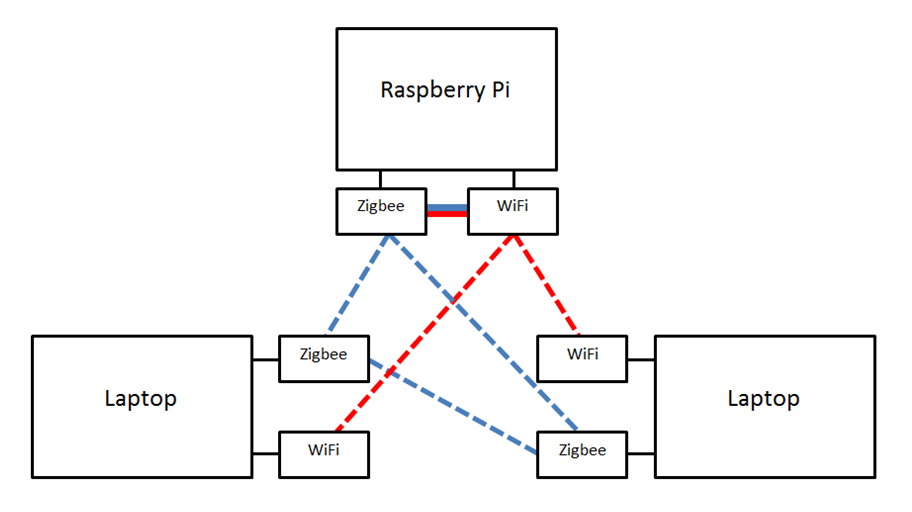
\includegraphics[width=\textwidth]{architectural-diagram}

\section{Components required}

\subsection{Already owned}

\begin{itemize}
  \item Raspberry Pi and laptops
  \item Two XBee Series 2 modules
  \item Two XBee RS232 boards
  \item Two USB-Serial converters
  \item Short ethernet cable
\end{itemize}

\subsection{To be bought}

\begin{itemize}
  \item One XBee Series 2 (ZB) module \url{https://www.coolcomponents.co.uk/xbee-2mw-module-with-whip-antenna-series-zb.html}
  \item One XBee USB board \url{https://www.coolcomponents.co.uk/xbee-explorer-usb-1460.html}
  \item One USB WiFi dongle \url{http://skpang.co.uk/catalog/miniature-wifi-80211bgn-module-for-raspberry-pi-p-1322.html}
\end{itemize}

\end{document}
